\begin{frame}{Objetivos}
    Desenvolver um modelo capaz de classificar diferentes imagens aéreas de acordo com o local que se referem.

    \begin{figure}
        \centering
        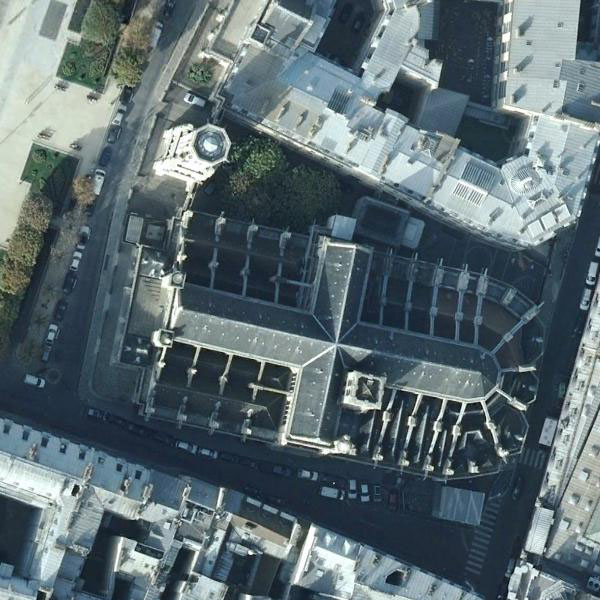
\includegraphics[width=0.35\linewidth]{AID/church_56.jpg}
        \caption{Visão aérea de uma igreja}
    \end{figure}
    
\end{frame}

\begin{frame}{Objetivos específicos}
    \begin{itemize}
        \item Explorar a literatura para identificar técnicas de classificação e \textit{datasets} disponíveis;
        \item Determinar um conjunto de dados para ser explorado;
        \item Propor, treinar e avaliar um modelo meio de métricas de acurácia global e outras métricas padronizadas de classificação;
        \item Comparar os resultados obtidos com os trabalhos relacionados;
        \item Identificar pontos fortes e limitações do método proposto, propondo diretrizes para futuras melhorias e ampliações do conjunto de dados e da arquitetura de classificação.
    \end{itemize}
\end{frame}